\chapter{Determining Plasma Flux Surfaces}

\label{chapter:flux}

This chapter goes over the flux surface coordinates that define the tokamak geometry. These are then used to approximate the surface area and volume, as well as create surface and volume integrals.

\begin{figure}[h]
	\centering
	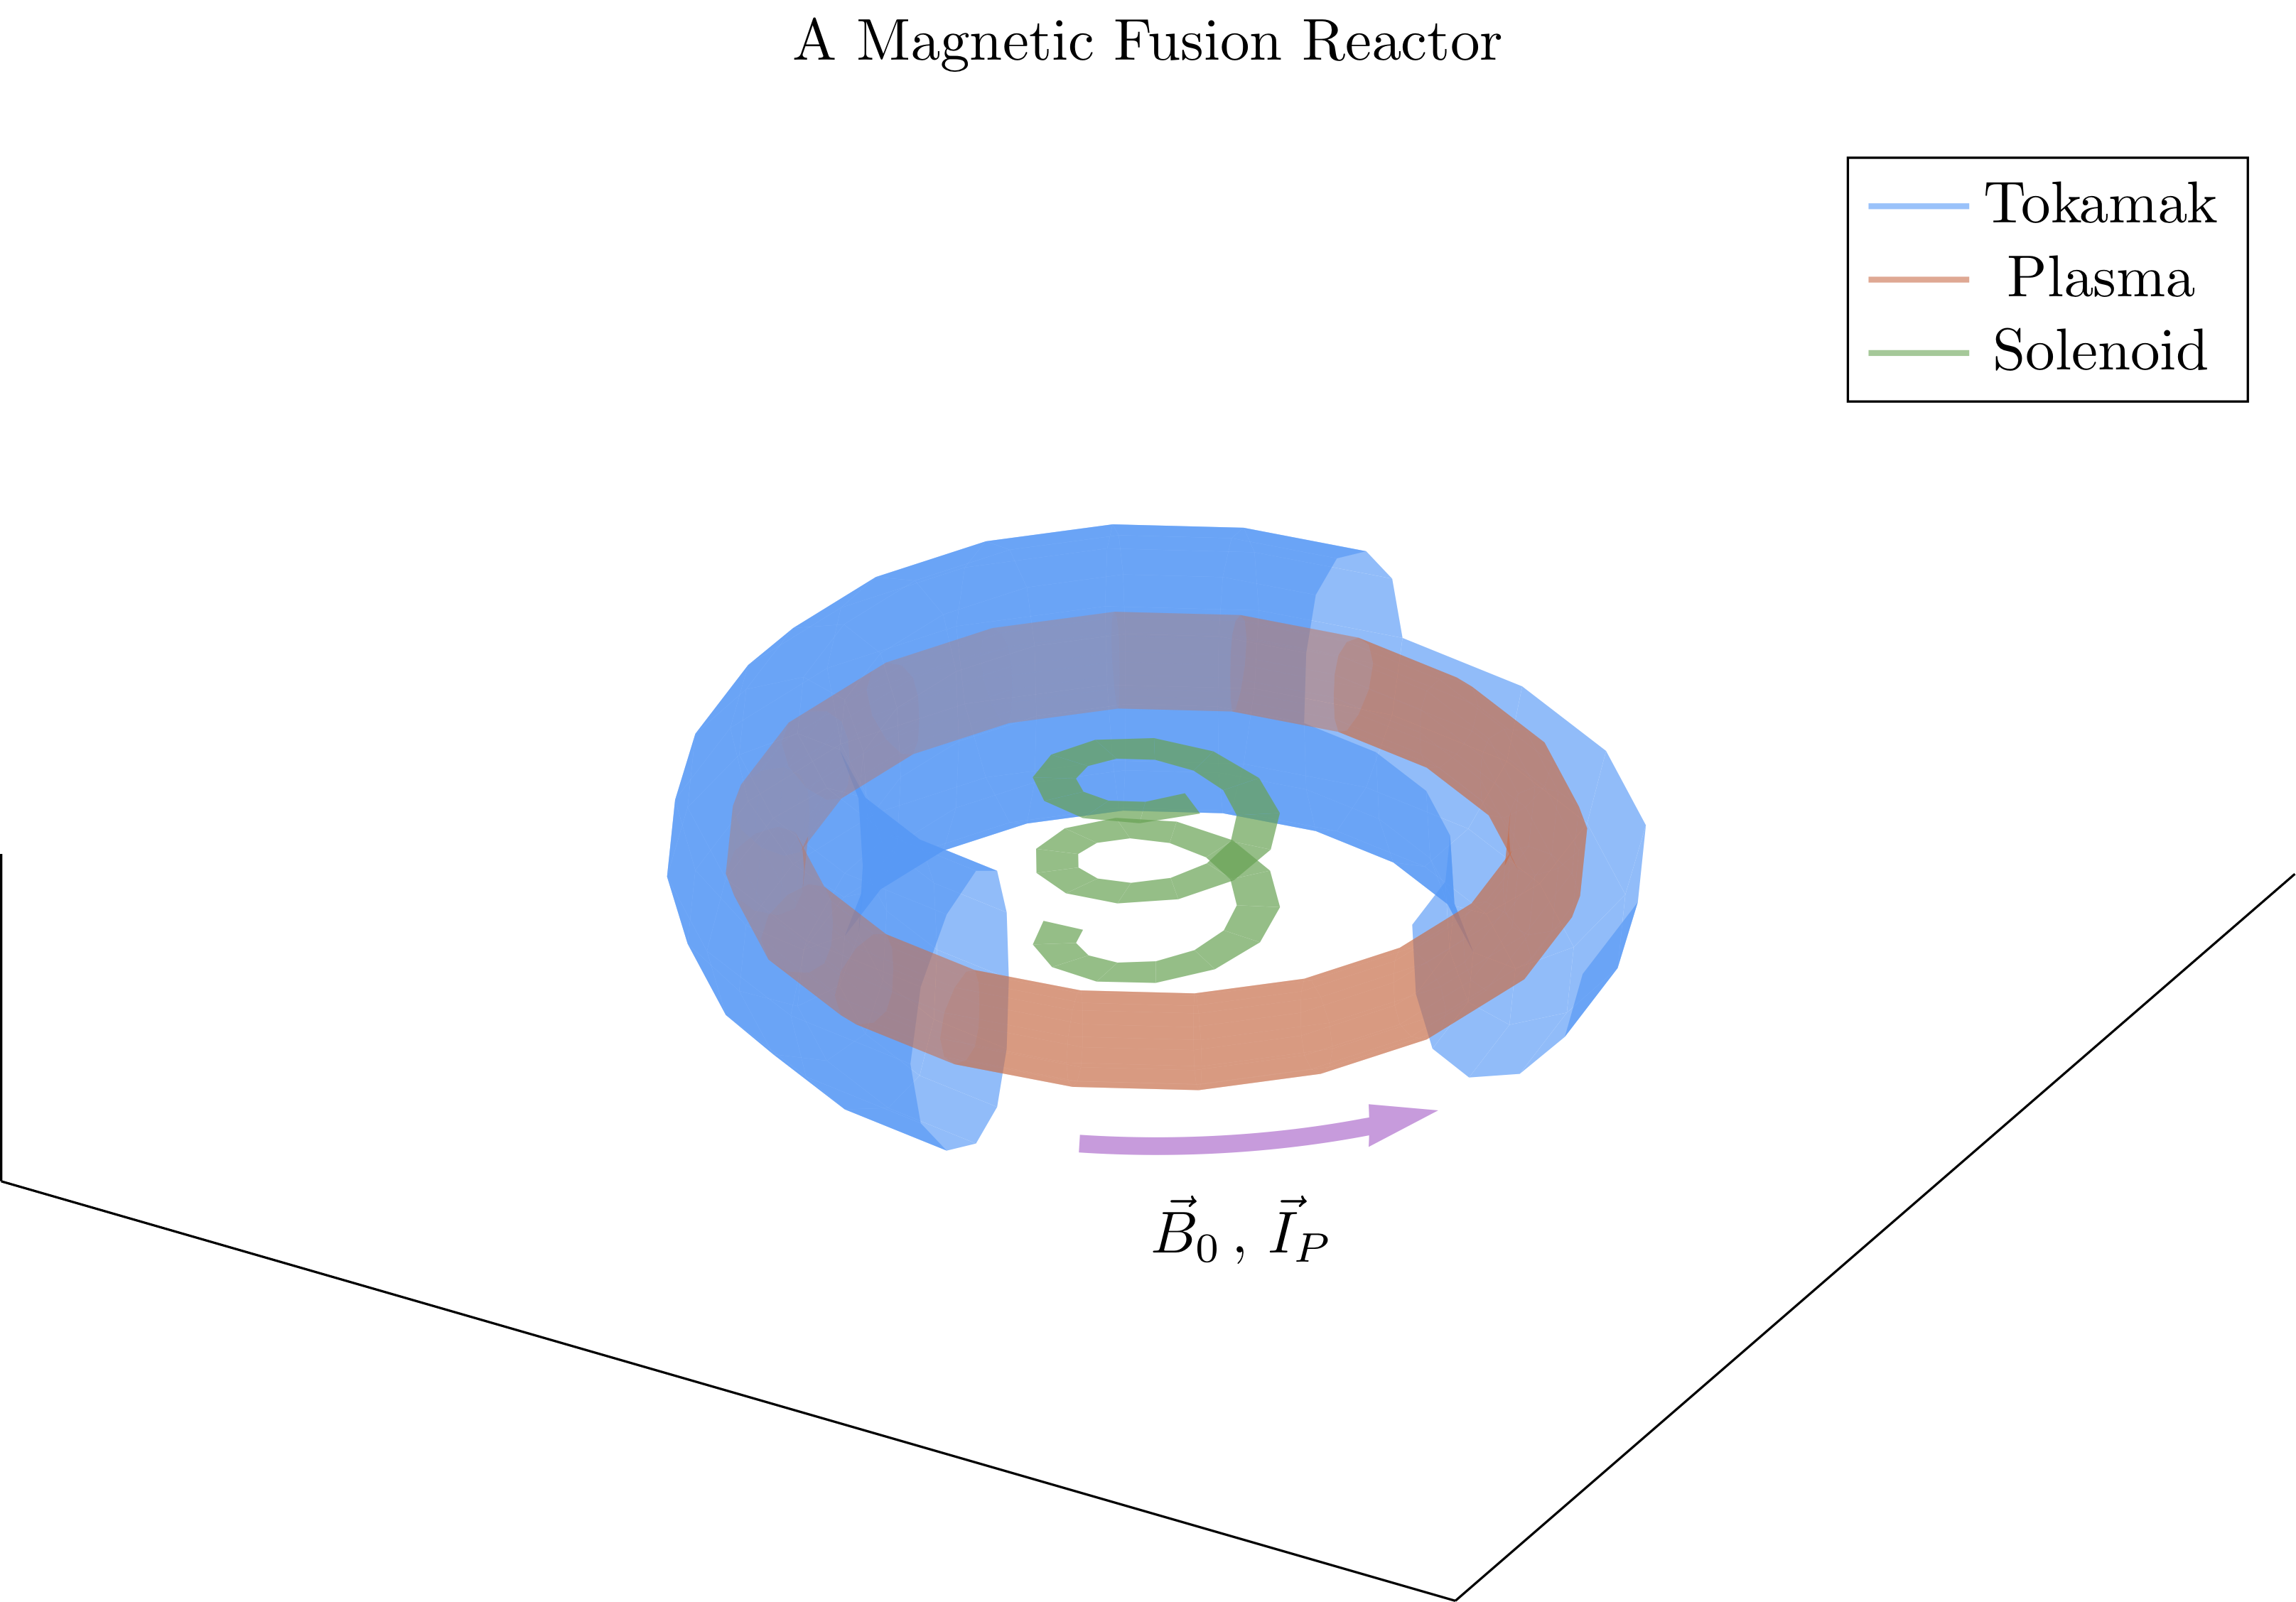
\includegraphics[width=0.85\textwidth]{images/fusion_reactor}
	\caption{Cut-Away of Tokamak Reactor} ~\\
	\small The three main components of a magnetic fusion reactor are: the tokamak structure, the plasma fuel, and the spring-like solenoid at the center.
\end{figure}

\section{Flux Surface Coordinates}

We begin with the shape of the outer plasma surface (i.e.\ the 95\% flux surface) written in terms of normalized coordinates x and y as follows -- with $\alpha$ being an angle-like coordinate:
\begin{gather}
	R = R_0 + a x( \alpha ) \\
	Z = a y( \alpha ) \\
	0 \le \alpha \le 2 \pi
\end{gather}
The surface representation can now be written as:
\begin{gather}
	\label{eq:xalpha}
	x(\alpha) = c_0 + c_1 \cos(\alpha) + c_2 \cos(2\alpha) + c_3 \cos(3\alpha) \\
	\label{eq:yalpha}
	y(\alpha) = \kappa \sin(\alpha)
\end{gather}
The constraints determining $c_j$ -- for $j = 1,2,3$ -- are chosen as:
\begin{gather}
	x(0) = 1 \\
	x(\pi) = -1 \\
	x\left(\frac{\pi}{2}\right) = -\delta \\
	x_{\alpha\alpha}(\pi) = 0.3 \cdot ( 1 - \delta ^2 )
\end{gather}
The last constraint, which is related to the surface curvature at $\alpha = \pi$, is chosen to make sure that the surface is always convex. A trial and error empirical fit resulted in the choice $x_{\alpha\alpha}(\pi) = 0.3 \cdot ( 1 - \delta ^2 )$. The constraint relations are easily evaluated and then solved, leading to values for the $c_j$,
\begin{gather}
	c_0 = { - \frac{ \delta }{ 2 } } \\
	c_1 = g \\
	c_2 = { \frac{ \delta }{ 2 } } \\
	c_3 = 1 - g
\end{gather}
Here, g is a shaping parameter approximately equal to one:
\begin{equation}
	g = \frac{9 - 2 \delta - 0.3 \cdot ( 1 - \delta ^2 ) }{8}
  \label{eq:gg}
\end{equation}
\myequations{Shaping Parameter -- $g$}

\section{Cross-sectional Area and Volume}

The plasma cross-sectional area and volume can be evaluated by straightforward calculations,
\begin{gather}
\begin{split}
	A & = \iint dR dZ = a^2 \iint dx dy = a^2 \int_0^{2 \pi} x \frac{dy}{d\alpha} d\alpha \\ & = \pi a^2 \kappa g
\end{split} \\
\begin{split}
	\volume & = \iiint R dR dZ d\Phi = 2 \pi a^2 \iint R dx dy \\ & = 2 \pi a^2 R_0 \int_0^{2 \pi} \left( x + \varepsilon \frac{ x^2 }{ 2} \right) \frac{dy}{d\alpha} d\alpha \approx 2 \pi a^2 R_0 \int_0^{2 \pi} x \frac{dy}{d\alpha} d\alpha \\ & = 2 \pi^2 R_0 a^2 \kappa g
\end{split}
\end{gather}
The second form of the volume integral makes use of the small inverse aspect ratio expansion, $\varepsilon \ll 1 $, which is a good approximation and used throughout the analysis.

\begin{figure*}[b]
\centering
\begin{adjustbox}{width=0.6\textwidth}
  \large
  \begin{adjustbox}{width=0.85\textwidth}
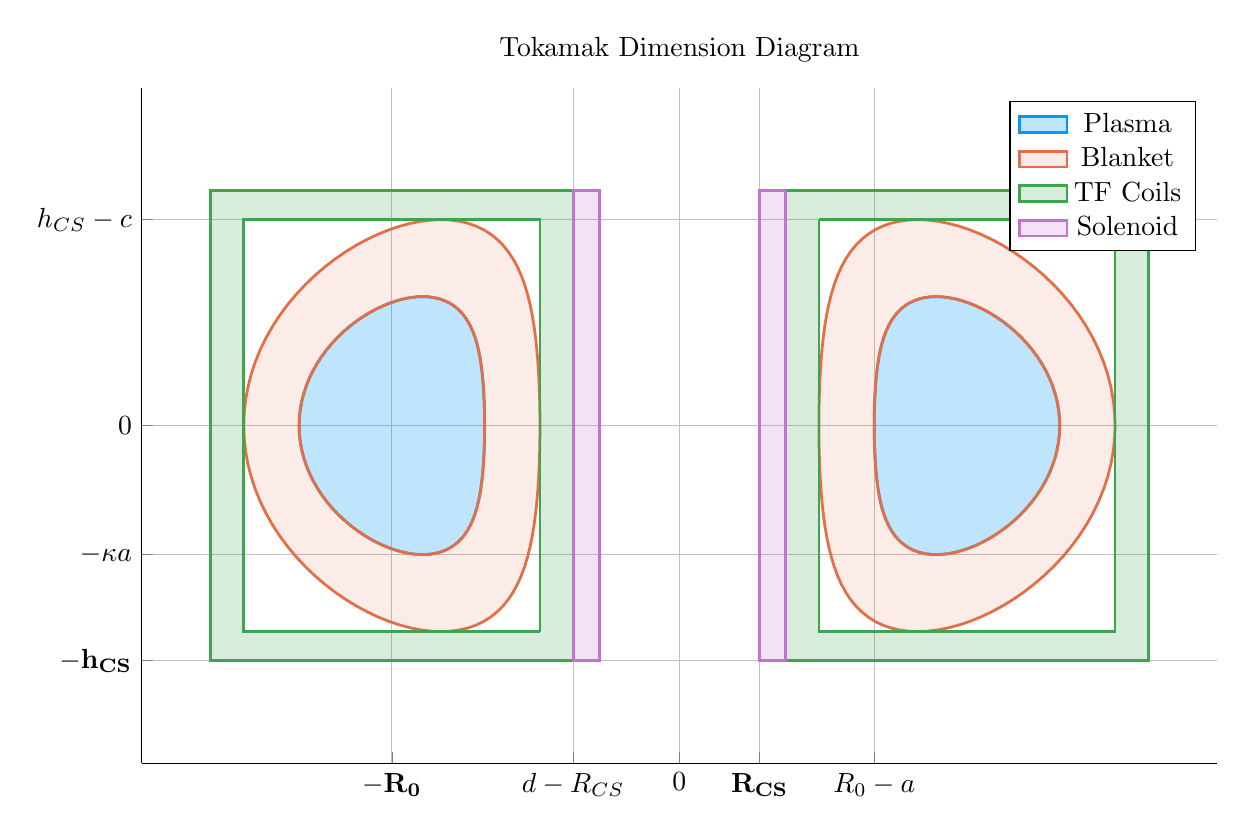
\begin{tikzpicture}[]
\begin{axis}[height = {101.6mm}, ylabel = {}, title = {Tokamak Dimension Diagram}, xmin = {-16.96464}, xmax = {16.96464}, ymax = {12.181706012903225}, xlabel = {}, unbounded coords=jump,scaled x ticks = false,xticklabel style={rotate = 0},xmajorgrids = true,xtick = {0.0,2.5317214541730677,-9.072,6.145548387096774,-3.3497214541730678},xticklabels = {0,$\bf{R_{CS}}$,$\bf{{-R}_0}$,$R_0 - a$,$d - R_{CS}$},xtick align = inside,axis lines* = left,scaled y ticks = false,yticklabel style={rotate = 0},ymajorgrids = true,ytick = {0.0,-8.478922887864822,-4.653058064516129,7.428922887864823},yticklabels = {0,$\bf{{-h}_{CS}}$,${-\kappa} a$,$h_{CS} - c$},ytick align = inside,axis lines* = left,    xshift = 0.0mm,
    yshift = 0.0mm,
    axis background/.style={fill={rgb,1:red,1.00000000;green,1.00000000;blue,1.00000000}}
, ymin = {-12.181706012903225}, width = {152.4mm}]\addplot+ [color = {rgb,1:red,0.00000000;green,0.60560316;blue,0.97868012},
draw opacity=1.0,
line width=1,
solid,mark = none,
mark size = 2.0,
mark options = {
    color = {rgb,1:red,0.00000000;green,0.00000000;blue,0.00000000}, draw opacity = 1.0,
    fill = {rgb,1:red,0.00000000;green,0.60560316;blue,0.97868012}, fill opacity = 1.0,
    line width = 1,
    rotate = 0,
    solid
},fill = {rgb,1:red,0.00000000;green,0.60560316;blue,0.97868012}, fill opacity=0.25,area legend]coordinates {
(-11.998451612903224, 0.0)
(-11.98922207919679, 0.2921679332710291)
(-11.961601612443932, 0.5831828131882695)
(-11.915794116436746, 0.8718961369727396)
(-11.852137762522407, 1.1571684850360338)
(-11.771102473770108, 1.4378740177488842)
(-11.673286377647635, 1.7129049186158334)
(-11.55941120568557, 1.9811757663208256)
(-11.430316617462449, 2.241627818389261)
(-11.286953428530017, 2.4932331895608506)
(-11.130375728034215, 2.7349989083831394)
(-10.96173188200961, 2.9659708360161865)
(-10.782254432669117, 3.1852374317826615)
(-10.59324892230544, 3.391933350602452)
(-10.396081692289423, 3.58524285811436)
(-10.192166732519574, 3.7644030500069485)
(-9.982951683794182, 3.9287068628533244)
(-9.769903124035281, 4.0775058645674545)
(-9.554491298062636, 4.21021281346937)
(-9.338174478579997, 4.326303975859794)
(-9.122383172034585, 4.425321192957779)
(-8.908504405883159, 4.5068736890441015)
(-8.697866352426912, 4.570639613674501)
(-8.491723557735288, 4.616367311876341)
(-8.2912430513685, 4.643876317315818)
(-8.097491612903225, 4.653058064516129)
(-7.911424464141755, 4.643876317315818)
(-7.73387564104738, 4.616367311876341)
(-7.565550276852846, 4.570639613674501)
(-7.4070189976483904, 4.506873689044102)
(-7.258714594546428, 4.42532119295778)
(-7.120931092970638, 4.326303975859795)
(-6.993825290693801, 4.21021281346937)
(-6.877420783129728, 4.077505864567455)
(-6.771614438426758, 3.928706862853325)
(-6.676185227609827, 3.7644030500069485)
(-6.590805257964794, 3.58524285811436)
(-6.515052802686304, 3.391933350602452)
(-6.448427068145589, 3.1852374317826624)
(-6.390364393542622, 2.9659708360161874)
(-6.340255537642832, 2.73499890838314)
(-6.297463675055492, 2.4932331895608506)
(-6.261342701178994, 2.241627818389261)
(-6.231255431364441, 1.9811757663208265)
(-6.206591276608178, 1.7129049186158343)
(-6.186782985455325, 1.4378740177488847)
(-6.171322059752492, 1.1571684850360338)
(-6.159772480089943, 0.8718961369727395)
(-6.151782414579849, 0.5831828131882707)
(-6.147093631099405, 0.29216793327103)
(-6.145548387096774, 5.698352664956456e-16)
(-6.147093631099405, -0.2921679332710289)
(-6.151782414579849, -0.5831828131882696)
(-6.159772480089943, -0.8718961369727383)
(-6.171322059752492, -1.1571684850360326)
(-6.1867829854553245, -1.4378740177488838)
(-6.206591276608178, -1.7129049186158334)
(-6.231255431364441, -1.9811757663208256)
(-6.261342701178992, -2.2416278183892597)
(-6.297463675055493, -2.4932331895608497)
(-6.340255537642832, -2.734998908383139)
(-6.390364393542622, -2.9659708360161865)
(-6.448427068145589, -3.185237431782662)
(-6.515052802686304, -3.3919333506024514)
(-6.590805257964794, -3.5852428581143605)
(-6.676185227609827, -3.7644030500069485)
(-6.771614438426755, -3.928706862853323)
(-6.877420783129727, -4.0775058645674545)
(-6.9938252906938, -4.21021281346937)
(-7.120931092970639, -4.326303975859795)
(-7.258714594546428, -4.425321192957779)
(-7.407018997648389, -4.5068736890441015)
(-7.565550276852846, -4.570639613674501)
(-7.733875641047377, -4.616367311876341)
(-7.9114244641417555, -4.643876317315818)
(-8.097491612903225, -4.653058064516129)
(-8.291243051368498, -4.643876317315818)
(-8.491723557735288, -4.616367311876341)
(-8.69786635242691, -4.570639613674501)
(-8.90850440588316, -4.5068736890441015)
(-9.122383172034585, -4.42532119295778)
(-9.338174478579994, -4.326303975859796)
(-9.554491298062636, -4.21021281346937)
(-9.76990312403528, -4.077505864567455)
(-9.982951683794184, -3.928706862853324)
(-10.192166732519574, -3.7644030500069494)
(-10.396081692289421, -3.5852428581143614)
(-10.59324892230544, -3.391933350602452)
(-10.782254432669115, -3.1852374317826624)
(-10.96173188200961, -2.9659708360161865)
(-11.130375728034215, -2.7349989083831403)
(-11.286953428530017, -2.493233189560853)
(-11.430316617462449, -2.241627818389261)
(-11.559411205685569, -1.981175766320827)
(-11.673286377647635, -1.7129049186158327)
(-11.771102473770108, -1.4378740177488853)
(-11.852137762522407, -1.1571684850360362)
(-11.915794116436746, -0.8718961369727398)
(-11.961601612443932, -0.5831828131882713)
(-11.98922207919679, -0.2921679332710286)
(-11.998451612903224, -1.1396705329912913e-15)
(NaN, NaN)
(11.998451612903224, 0.0)
(11.98922207919679, 0.2921679332710291)
(11.961601612443932, 0.5831828131882695)
(11.915794116436746, 0.8718961369727396)
(11.852137762522407, 1.1571684850360338)
(11.771102473770108, 1.4378740177488842)
(11.673286377647635, 1.7129049186158334)
(11.55941120568557, 1.9811757663208256)
(11.430316617462449, 2.241627818389261)
(11.286953428530017, 2.4932331895608506)
(11.130375728034215, 2.7349989083831394)
(10.96173188200961, 2.9659708360161865)
(10.782254432669117, 3.1852374317826615)
(10.59324892230544, 3.391933350602452)
(10.396081692289423, 3.58524285811436)
(10.192166732519574, 3.7644030500069485)
(9.982951683794182, 3.9287068628533244)
(9.769903124035281, 4.0775058645674545)
(9.554491298062636, 4.21021281346937)
(9.338174478579997, 4.326303975859794)
(9.122383172034585, 4.425321192957779)
(8.908504405883159, 4.5068736890441015)
(8.697866352426912, 4.570639613674501)
(8.491723557735288, 4.616367311876341)
(8.2912430513685, 4.643876317315818)
(8.097491612903225, 4.653058064516129)
(7.911424464141755, 4.643876317315818)
(7.73387564104738, 4.616367311876341)
(7.565550276852846, 4.570639613674501)
(7.4070189976483904, 4.506873689044102)
(7.258714594546428, 4.42532119295778)
(7.120931092970638, 4.326303975859795)
(6.993825290693801, 4.21021281346937)
(6.877420783129728, 4.077505864567455)
(6.771614438426758, 3.928706862853325)
(6.676185227609827, 3.7644030500069485)
(6.590805257964794, 3.58524285811436)
(6.515052802686304, 3.391933350602452)
(6.448427068145589, 3.1852374317826624)
(6.390364393542622, 2.9659708360161874)
(6.340255537642832, 2.73499890838314)
(6.297463675055492, 2.4932331895608506)
(6.261342701178994, 2.241627818389261)
(6.231255431364441, 1.9811757663208265)
(6.206591276608178, 1.7129049186158343)
(6.186782985455325, 1.4378740177488847)
(6.171322059752492, 1.1571684850360338)
(6.159772480089943, 0.8718961369727395)
(6.151782414579849, 0.5831828131882707)
(6.147093631099405, 0.29216793327103)
(6.145548387096774, 5.698352664956456e-16)
(6.147093631099405, -0.2921679332710289)
(6.151782414579849, -0.5831828131882696)
(6.159772480089943, -0.8718961369727383)
(6.171322059752492, -1.1571684850360326)
(6.1867829854553245, -1.4378740177488838)
(6.206591276608178, -1.7129049186158334)
(6.231255431364441, -1.9811757663208256)
(6.261342701178992, -2.2416278183892597)
(6.297463675055493, -2.4932331895608497)
(6.340255537642832, -2.734998908383139)
(6.390364393542622, -2.9659708360161865)
(6.448427068145589, -3.185237431782662)
(6.515052802686304, -3.3919333506024514)
(6.590805257964794, -3.5852428581143605)
(6.676185227609827, -3.7644030500069485)
(6.771614438426755, -3.928706862853323)
(6.877420783129727, -4.0775058645674545)
(6.9938252906938, -4.21021281346937)
(7.120931092970639, -4.326303975859795)
(7.258714594546428, -4.425321192957779)
(7.407018997648389, -4.5068736890441015)
(7.565550276852846, -4.570639613674501)
(7.733875641047377, -4.616367311876341)
(7.9114244641417555, -4.643876317315818)
(8.097491612903225, -4.653058064516129)
(8.291243051368498, -4.643876317315818)
(8.491723557735288, -4.616367311876341)
(8.69786635242691, -4.570639613674501)
(8.90850440588316, -4.5068736890441015)
(9.122383172034585, -4.42532119295778)
(9.338174478579994, -4.326303975859796)
(9.554491298062636, -4.21021281346937)
(9.76990312403528, -4.077505864567455)
(9.982951683794184, -3.928706862853324)
(10.192166732519574, -3.7644030500069494)
(10.396081692289421, -3.5852428581143614)
(10.59324892230544, -3.391933350602452)
(10.782254432669115, -3.1852374317826624)
(10.96173188200961, -2.9659708360161865)
(11.130375728034215, -2.7349989083831403)
(11.286953428530017, -2.493233189560853)
(11.430316617462449, -2.241627818389261)
(11.559411205685569, -1.981175766320827)
(11.673286377647635, -1.7129049186158327)
(11.771102473770108, -1.4378740177488853)
(11.852137762522407, -1.1571684850360362)
(11.915794116436746, -0.8718961369727398)
(11.961601612443932, -0.5831828131882713)
(11.98922207919679, -0.2921679332710286)
(11.998451612903224, -1.1396705329912913e-15)
};
\addlegendentry{Plasma}
\addplot+ [color = {rgb,1:red,0.88887350;green,0.43564919;blue,0.27812294},
draw opacity=1.0,
line width=1,
solid,mark = none,
mark size = 2.0,
mark options = {
    color = {rgb,1:red,0.00000000;green,0.00000000;blue,0.00000000}, draw opacity = 1.0,
    fill = {rgb,1:red,0.88887350;green,0.43564919;blue,0.27812294}, fill opacity = 1.0,
    line width = 1,
    rotate = 0,
    solid
},fill = {rgb,1:red,0.88887350;green,0.43564919;blue,0.27812294}, fill opacity=0.125,area legend]coordinates {
(-13.74427854582693, 0.0)
(-13.72954296908463, 0.46646592767223927)
(-13.685445019996358, 0.9310909274359673)
(-13.612310244800092, 1.392041336684088)
(-13.510678556994915, 1.8474979947395098)
(-13.381300220642846, 2.2956634222512418)
(-13.225130186826302, 2.734768915024204)
(-13.04332074889991, 3.1630815242866377)
(-12.837212480347718, 3.5789108958472036)
(-12.608323422706404, 3.9806159411507194)
(-12.358336500812388, 4.3666113139049525)
(-12.08908515895104, 4.735373666718153)
(-11.802537234387401, 5.08544766305526)
(-11.500777113966619, 5.4154517207863275)
(-11.185986254387002, 5.724083464660006)
(-10.860422186454013, 6.010124866183653)
(-10.526396166917667, 6.272447050625345)
(-10.18624968693083, 6.510014752166694)
(-9.842330092097374, 6.721890399624077)
(-9.496965613725703, 6.907237816613755)
(-9.152440152411872, 7.065325521558049)
(-8.81096819159381, 7.195529614508949)
(-8.474670248460548, 7.297336239396166)
(-8.14554929092694, 7.370343611982296)
(-7.825468560863273, 7.4142636055216355)
(-7.516131244239631, 7.428922887864823)
(-7.2190624174706315, 7.4142636055216355)
(-6.935593675557043, 7.370343611982296)
(-6.666850811544881, 7.297336239396167)
(-6.4137448687014755, 7.195529614508949)
(-6.176966827400615, 7.065325521558051)
(-5.956986119179431, 6.907237816613756)
(-5.754053082320152, 6.721890399624076)
(-5.568205388501765, 6.510014752166695)
(-5.3992783807260825, 6.272447050625345)
(-5.246919171238659, 6.010124866183653)
(-5.110604257075394, 5.724083464660006)
(-4.989660322779391, 5.4154517207863275)
(-4.88328781734585, 5.085447663055262)
(-4.790586818065825, 4.735373666718154)
(-4.7105846299742, 4.366611313904953)
(-4.642264518129107, 3.9806159411507194)
(-4.584594932698949, 3.578910895847203)
(-4.536558565161822, 3.1630815242866395)
(-4.497180568747824, 2.7347689150242047)
(-4.465555288023927, 2.2956634222512426)
(-4.440870871189059, 1.8474979947395103)
(-4.422431183673739, 1.3920413366840876)
(-4.409674501998921, 0.9310909274359696)
(-4.402188541060726, 0.46646592767224077)
(-4.399721454173068, 9.097806635736167e-16)
(-4.402188541060726, -0.466465927672239)
(-4.409674501998921, -0.9310909274359678)
(-4.422431183673739, -1.392041336684086)
(-4.440870871189059, -1.8474979947395083)
(-4.465555288023926, -2.295663422251241)
(-4.497180568747823, -2.734768915024204)
(-4.536558565161822, -3.1630815242866377)
(-4.5845949326989475, -3.5789108958472013)
(-4.642264518129108, -3.980615941150719)
(-4.7105846299742, -4.3666113139049525)
(-4.790586818065825, -4.735373666718153)
(-4.88328781734585, -5.085447663055261)
(-4.989660322779391, -5.415451720786327)
(-5.110604257075395, -5.724083464660007)
(-5.246919171238659, -6.010124866183653)
(-5.399278380726081, -6.272447050625343)
(-5.568205388501764, -6.510014752166694)
(-5.754053082320152, -6.721890399624076)
(-5.956986119179432, -6.907237816613756)
(-6.176966827400615, -7.065325521558049)
(-6.413744868701472, -7.195529614508947)
(-6.666850811544881, -7.297336239396167)
(-6.935593675557041, -7.370343611982296)
(-7.219062417470632, -7.4142636055216355)
(-7.51613124423963, -7.428922887864823)
(-7.8254685608632695, -7.4142636055216355)
(-8.14554929092694, -7.370343611982296)
(-8.474670248460544, -7.297336239396167)
(-8.810968191593812, -7.195529614508949)
(-9.152440152411872, -7.065325521558051)
(-9.4969656137257, -6.9072378166137565)
(-9.842330092097372, -6.721890399624077)
(-10.186249686930825, -6.510014752166696)
(-10.526396166917669, -6.272447050625344)
(-10.860422186454013, -6.010124866183654)
(-11.185986254386998, -5.724083464660007)
(-11.500777113966619, -5.4154517207863275)
(-11.8025372343874, -5.085447663055262)
(-12.08908515895104, -4.735373666718153)
(-12.358336500812388, -4.366611313904954)
(-12.608323422706402, -3.9806159411507234)
(-12.837212480347718, -3.5789108958472036)
(-13.04332074889991, -3.1630815242866404)
(-13.225130186826302, -2.7347689150242034)
(-13.381300220642846, -2.2956634222512435)
(-13.510678556994915, -1.8474979947395136)
(-13.612310244800092, -1.3920413366840885)
(-13.685445019996358, -0.9310909274359703)
(-13.72954296908463, -0.46646592767223843)
(-13.74427854582693, -1.8195613271472333e-15)
(NaN, NaN)
(13.74427854582693, 0.0)
(13.72954296908463, 0.46646592767223927)
(13.685445019996358, 0.9310909274359673)
(13.612310244800092, 1.392041336684088)
(13.510678556994915, 1.8474979947395098)
(13.381300220642846, 2.2956634222512418)
(13.225130186826302, 2.734768915024204)
(13.04332074889991, 3.1630815242866377)
(12.837212480347718, 3.5789108958472036)
(12.608323422706404, 3.9806159411507194)
(12.358336500812388, 4.3666113139049525)
(12.08908515895104, 4.735373666718153)
(11.802537234387401, 5.08544766305526)
(11.500777113966619, 5.4154517207863275)
(11.185986254387002, 5.724083464660006)
(10.860422186454013, 6.010124866183653)
(10.526396166917667, 6.272447050625345)
(10.18624968693083, 6.510014752166694)
(9.842330092097374, 6.721890399624077)
(9.496965613725703, 6.907237816613755)
(9.152440152411872, 7.065325521558049)
(8.81096819159381, 7.195529614508949)
(8.474670248460548, 7.297336239396166)
(8.14554929092694, 7.370343611982296)
(7.825468560863273, 7.4142636055216355)
(7.516131244239631, 7.428922887864823)
(7.2190624174706315, 7.4142636055216355)
(6.935593675557043, 7.370343611982296)
(6.666850811544881, 7.297336239396167)
(6.4137448687014755, 7.195529614508949)
(6.176966827400615, 7.065325521558051)
(5.956986119179431, 6.907237816613756)
(5.754053082320152, 6.721890399624076)
(5.568205388501765, 6.510014752166695)
(5.3992783807260825, 6.272447050625345)
(5.246919171238659, 6.010124866183653)
(5.110604257075394, 5.724083464660006)
(4.989660322779391, 5.4154517207863275)
(4.88328781734585, 5.085447663055262)
(4.790586818065825, 4.735373666718154)
(4.7105846299742, 4.366611313904953)
(4.642264518129107, 3.9806159411507194)
(4.584594932698949, 3.578910895847203)
(4.536558565161822, 3.1630815242866395)
(4.497180568747824, 2.7347689150242047)
(4.465555288023927, 2.2956634222512426)
(4.440870871189059, 1.8474979947395103)
(4.422431183673739, 1.3920413366840876)
(4.409674501998921, 0.9310909274359696)
(4.402188541060726, 0.46646592767224077)
(4.399721454173068, 9.097806635736167e-16)
(4.402188541060726, -0.466465927672239)
(4.409674501998921, -0.9310909274359678)
(4.422431183673739, -1.392041336684086)
(4.440870871189059, -1.8474979947395083)
(4.465555288023926, -2.295663422251241)
(4.497180568747823, -2.734768915024204)
(4.536558565161822, -3.1630815242866377)
(4.5845949326989475, -3.5789108958472013)
(4.642264518129108, -3.980615941150719)
(4.7105846299742, -4.3666113139049525)
(4.790586818065825, -4.735373666718153)
(4.88328781734585, -5.085447663055261)
(4.989660322779391, -5.415451720786327)
(5.110604257075395, -5.724083464660007)
(5.246919171238659, -6.010124866183653)
(5.399278380726081, -6.272447050625343)
(5.568205388501764, -6.510014752166694)
(5.754053082320152, -6.721890399624076)
(5.956986119179432, -6.907237816613756)
(6.176966827400615, -7.065325521558049)
(6.413744868701472, -7.195529614508947)
(6.666850811544881, -7.297336239396167)
(6.935593675557041, -7.370343611982296)
(7.219062417470632, -7.4142636055216355)
(7.51613124423963, -7.428922887864823)
(7.8254685608632695, -7.4142636055216355)
(8.14554929092694, -7.370343611982296)
(8.474670248460544, -7.297336239396167)
(8.810968191593812, -7.195529614508949)
(9.152440152411872, -7.065325521558051)
(9.4969656137257, -6.9072378166137565)
(9.842330092097372, -6.721890399624077)
(10.186249686930825, -6.510014752166696)
(10.526396166917669, -6.272447050625344)
(10.860422186454013, -6.010124866183654)
(11.185986254386998, -5.724083464660007)
(11.500777113966619, -5.4154517207863275)
(11.8025372343874, -5.085447663055262)
(12.08908515895104, -4.735373666718153)
(12.358336500812388, -4.366611313904954)
(12.608323422706402, -3.9806159411507234)
(12.837212480347718, -3.5789108958472036)
(13.04332074889991, -3.1630815242866404)
(13.225130186826302, -2.7347689150242034)
(13.381300220642846, -2.2956634222512435)
(13.510678556994915, -1.8474979947395136)
(13.612310244800092, -1.3920413366840885)
(13.685445019996358, -0.9310909274359703)
(13.72954296908463, -0.46646592767223843)
(13.74427854582693, -1.8195613271472333e-15)
(NaN, NaN)
(11.998451612903224, -1.1396705329912913e-15)
(11.98922207919679, -0.2921679332710286)
(11.961601612443932, -0.5831828131882713)
(11.915794116436746, -0.8718961369727398)
(11.852137762522407, -1.1571684850360362)
(11.771102473770108, -1.4378740177488853)
(11.673286377647635, -1.7129049186158327)
(11.55941120568557, -1.981175766320827)
(11.430316617462449, -2.241627818389261)
(11.286953428530017, -2.493233189560853)
(11.130375728034215, -2.7349989083831403)
(10.96173188200961, -2.9659708360161865)
(10.782254432669117, -3.1852374317826624)
(10.59324892230544, -3.391933350602452)
(10.396081692289423, -3.5852428581143614)
(10.192166732519574, -3.7644030500069494)
(9.982951683794182, -3.928706862853324)
(9.769903124035281, -4.077505864567455)
(9.554491298062636, -4.21021281346937)
(9.338174478579997, -4.326303975859796)
(9.122383172034585, -4.42532119295778)
(8.908504405883159, -4.5068736890441015)
(8.697866352426912, -4.570639613674501)
(8.491723557735288, -4.616367311876341)
(8.2912430513685, -4.643876317315818)
(8.097491612903225, -4.653058064516129)
(7.911424464141755, -4.643876317315818)
(7.73387564104738, -4.616367311876341)
(7.565550276852846, -4.570639613674501)
(7.4070189976483904, -4.5068736890441015)
(7.258714594546428, -4.425321192957779)
(7.120931092970638, -4.326303975859795)
(6.993825290693801, -4.21021281346937)
(6.877420783129728, -4.0775058645674545)
(6.771614438426758, -3.928706862853323)
(6.676185227609827, -3.7644030500069485)
(6.590805257964794, -3.5852428581143605)
(6.515052802686304, -3.3919333506024514)
(6.448427068145589, -3.185237431782662)
(6.390364393542622, -2.9659708360161865)
(6.340255537642832, -2.734998908383139)
(6.297463675055492, -2.4932331895608497)
(6.261342701178994, -2.2416278183892597)
(6.231255431364441, -1.9811757663208256)
(6.206591276608178, -1.7129049186158334)
(6.186782985455325, -1.4378740177488838)
(6.171322059752492, -1.1571684850360326)
(6.159772480089943, -0.8718961369727383)
(6.151782414579849, -0.5831828131882696)
(6.147093631099405, -0.2921679332710289)
(6.145548387096774, 5.698352664956456e-16)
(6.147093631099405, 0.29216793327103)
(6.151782414579849, 0.5831828131882707)
(6.159772480089943, 0.8718961369727395)
(6.171322059752492, 1.1571684850360338)
(6.1867829854553245, 1.4378740177488847)
(6.206591276608178, 1.7129049186158343)
(6.231255431364441, 1.9811757663208265)
(6.261342701178992, 2.241627818389261)
(6.297463675055493, 2.4932331895608506)
(6.340255537642832, 2.73499890838314)
(6.390364393542622, 2.9659708360161874)
(6.448427068145589, 3.1852374317826624)
(6.515052802686304, 3.391933350602452)
(6.590805257964794, 3.58524285811436)
(6.676185227609827, 3.7644030500069485)
(6.771614438426755, 3.928706862853325)
(6.877420783129727, 4.077505864567455)
(6.9938252906938, 4.21021281346937)
(7.120931092970639, 4.326303975859795)
(7.258714594546428, 4.42532119295778)
(7.407018997648389, 4.506873689044102)
(7.565550276852846, 4.570639613674501)
(7.733875641047377, 4.616367311876341)
(7.9114244641417555, 4.643876317315818)
(8.097491612903225, 4.653058064516129)
(8.291243051368498, 4.643876317315818)
(8.491723557735288, 4.616367311876341)
(8.69786635242691, 4.570639613674501)
(8.90850440588316, 4.5068736890441015)
(9.122383172034585, 4.425321192957779)
(9.338174478579994, 4.326303975859794)
(9.554491298062636, 4.21021281346937)
(9.76990312403528, 4.0775058645674545)
(9.982951683794184, 3.9287068628533244)
(10.192166732519574, 3.7644030500069485)
(10.396081692289421, 3.58524285811436)
(10.59324892230544, 3.391933350602452)
(10.782254432669115, 3.1852374317826615)
(10.96173188200961, 2.9659708360161865)
(11.130375728034215, 2.7349989083831394)
(11.286953428530017, 2.4932331895608506)
(11.430316617462449, 2.241627818389261)
(11.559411205685569, 1.9811757663208256)
(11.673286377647635, 1.7129049186158334)
(11.771102473770108, 1.4378740177488842)
(11.852137762522407, 1.1571684850360338)
(11.915794116436746, 0.8718961369727396)
(11.961601612443932, 0.5831828131882695)
(11.98922207919679, 0.2921679332710291)
(11.998451612903224, 0.0)
(NaN, NaN)
(-11.998451612903224, -1.1396705329912913e-15)
(-11.98922207919679, -0.2921679332710286)
(-11.961601612443932, -0.5831828131882713)
(-11.915794116436746, -0.8718961369727398)
(-11.852137762522407, -1.1571684850360362)
(-11.771102473770108, -1.4378740177488853)
(-11.673286377647635, -1.7129049186158327)
(-11.55941120568557, -1.981175766320827)
(-11.430316617462449, -2.241627818389261)
(-11.286953428530017, -2.493233189560853)
(-11.130375728034215, -2.7349989083831403)
(-10.96173188200961, -2.9659708360161865)
(-10.782254432669117, -3.1852374317826624)
(-10.59324892230544, -3.391933350602452)
(-10.396081692289423, -3.5852428581143614)
(-10.192166732519574, -3.7644030500069494)
(-9.982951683794182, -3.928706862853324)
(-9.769903124035281, -4.077505864567455)
(-9.554491298062636, -4.21021281346937)
(-9.338174478579997, -4.326303975859796)
(-9.122383172034585, -4.42532119295778)
(-8.908504405883159, -4.5068736890441015)
(-8.697866352426912, -4.570639613674501)
(-8.491723557735288, -4.616367311876341)
(-8.2912430513685, -4.643876317315818)
(-8.097491612903225, -4.653058064516129)
(-7.911424464141755, -4.643876317315818)
(-7.73387564104738, -4.616367311876341)
(-7.565550276852846, -4.570639613674501)
(-7.4070189976483904, -4.5068736890441015)
(-7.258714594546428, -4.425321192957779)
(-7.120931092970638, -4.326303975859795)
(-6.993825290693801, -4.21021281346937)
(-6.877420783129728, -4.0775058645674545)
(-6.771614438426758, -3.928706862853323)
(-6.676185227609827, -3.7644030500069485)
(-6.590805257964794, -3.5852428581143605)
(-6.515052802686304, -3.3919333506024514)
(-6.448427068145589, -3.185237431782662)
(-6.390364393542622, -2.9659708360161865)
(-6.340255537642832, -2.734998908383139)
(-6.297463675055492, -2.4932331895608497)
(-6.261342701178994, -2.2416278183892597)
(-6.231255431364441, -1.9811757663208256)
(-6.206591276608178, -1.7129049186158334)
(-6.186782985455325, -1.4378740177488838)
(-6.171322059752492, -1.1571684850360326)
(-6.159772480089943, -0.8718961369727383)
(-6.151782414579849, -0.5831828131882696)
(-6.147093631099405, -0.2921679332710289)
(-6.145548387096774, 5.698352664956456e-16)
(-6.147093631099405, 0.29216793327103)
(-6.151782414579849, 0.5831828131882707)
(-6.159772480089943, 0.8718961369727395)
(-6.171322059752492, 1.1571684850360338)
(-6.1867829854553245, 1.4378740177488847)
(-6.206591276608178, 1.7129049186158343)
(-6.231255431364441, 1.9811757663208265)
(-6.261342701178992, 2.241627818389261)
(-6.297463675055493, 2.4932331895608506)
(-6.340255537642832, 2.73499890838314)
(-6.390364393542622, 2.9659708360161874)
(-6.448427068145589, 3.1852374317826624)
(-6.515052802686304, 3.391933350602452)
(-6.590805257964794, 3.58524285811436)
(-6.676185227609827, 3.7644030500069485)
(-6.771614438426755, 3.928706862853325)
(-6.877420783129727, 4.077505864567455)
(-6.9938252906938, 4.21021281346937)
(-7.120931092970639, 4.326303975859795)
(-7.258714594546428, 4.42532119295778)
(-7.407018997648389, 4.506873689044102)
(-7.565550276852846, 4.570639613674501)
(-7.733875641047377, 4.616367311876341)
(-7.9114244641417555, 4.643876317315818)
(-8.097491612903225, 4.653058064516129)
(-8.291243051368498, 4.643876317315818)
(-8.491723557735288, 4.616367311876341)
(-8.69786635242691, 4.570639613674501)
(-8.90850440588316, 4.5068736890441015)
(-9.122383172034585, 4.425321192957779)
(-9.338174478579994, 4.326303975859794)
(-9.554491298062636, 4.21021281346937)
(-9.76990312403528, 4.0775058645674545)
(-9.982951683794184, 3.9287068628533244)
(-10.192166732519574, 3.7644030500069485)
(-10.396081692289421, 3.58524285811436)
(-10.59324892230544, 3.391933350602452)
(-10.782254432669115, 3.1852374317826615)
(-10.96173188200961, 2.9659708360161865)
(-11.130375728034215, 2.7349989083831394)
(-11.286953428530017, 2.4932331895608506)
(-11.430316617462449, 2.241627818389261)
(-11.559411205685569, 1.9811757663208256)
(-11.673286377647635, 1.7129049186158334)
(-11.771102473770108, 1.4378740177488842)
(-11.852137762522407, 1.1571684850360338)
(-11.915794116436746, 0.8718961369727396)
(-11.961601612443932, 0.5831828131882695)
(-11.98922207919679, 0.2921679332710291)
(-11.998451612903224, 0.0)
};
\addlegendentry{Blanket}
\addplot+ [color = {rgb,1:red,0.24222430;green,0.64327509;blue,0.30444865},
draw opacity=1.0,
line width=1,
solid,mark = none,
mark size = 2.0,
mark options = {
    color = {rgb,1:red,0.00000000;green,0.00000000;blue,0.00000000}, draw opacity = 1.0,
    fill = {rgb,1:red,0.24222430;green,0.64327509;blue,0.30444865}, fill opacity = 1.0,
    line width = 1,
    rotate = 0,
    solid
},fill = {rgb,1:red,0.24222430;green,0.64327509;blue,0.30444865}, fill opacity=0.2,area legend]coordinates {
(-4.399721454173068, -7.428922887864823)
(-13.74427854582693, -7.428922887864823)
(-13.74427854582693, 7.428922887864823)
(-4.399721454173068, 7.428922887864823)
(-4.399721454173068, -7.428922887864823)
(NaN, NaN)
(-3.3497214541730678, -8.478922887864822)
(-3.3497214541730678, 8.478922887864822)
(-14.79427854582693, 8.478922887864822)
(-14.79427854582693, -8.478922887864822)
(-3.3497214541730678, -8.478922887864822)
(NaN, NaN)
(4.399721454173068, 7.428922887864823)
(13.74427854582693, 7.428922887864823)
(13.74427854582693, -7.428922887864823)
(4.399721454173068, -7.428922887864823)
(4.399721454173068, 7.428922887864823)
(NaN, NaN)
(3.3497214541730678, 8.478922887864822)
(3.3497214541730678, -8.478922887864822)
(14.79427854582693, -8.478922887864822)
(14.79427854582693, 8.478922887864822)
(3.3497214541730678, 8.478922887864822)
};
\addlegendentry{TF Coils}
\addplot+ [color = {rgb,1:red,0.76444018;green,0.44411178;blue,0.82429754},
draw opacity=1.0,
line width=1,
solid,mark = none,
mark size = 2.0,
mark options = {
    color = {rgb,1:red,0.00000000;green,0.00000000;blue,0.00000000}, draw opacity = 1.0,
    fill = {rgb,1:red,0.76444018;green,0.44411178;blue,0.82429754}, fill opacity = 1.0,
    line width = 1,
    rotate = 0,
    solid
},fill = {rgb,1:red,0.76444018;green,0.44411178;blue,0.82429754}, fill opacity=0.2,area legend]coordinates {
(-3.3497214541730678, -8.478922887864822)
(-3.3497214541730678, 8.478922887864822)
(-2.5317214541730677, 8.478922887864822)
(-2.5317214541730677, -8.478922887864822)
(-3.3497214541730678, -8.478922887864822)
(NaN, NaN)
(3.3497214541730678, 8.478922887864822)
(3.3497214541730678, -8.478922887864822)
(2.5317214541730677, -8.478922887864822)
(2.5317214541730677, 8.478922887864822)
(3.3497214541730678, 8.478922887864822)
};
\addlegendentry{Solenoid}
\end{axis}

\end{tikzpicture}

\end{adjustbox}

\end{adjustbox}
\caption{Dimensions of Tokamak Cross-Section}
\label{fig:dims}
\end{figure*}

\section{Surface and Volume Integrals}

\cref{eq:xalpha,eq:yalpha} are simple formulas describing the shape of the outer plasma surface. We next modify the model so that it gives a plausible description of the interior flux surfaces as well. The idea is to introduce a normalized flux label, which is radial-like in behavior. This label is denoted by $\rho$ and $\rho \in [0,1]$ with $\rho = 1$ being the outer plasma surface (i.e.\ the 95\% surface) and $\rho = 0$ being the magnetic axis. Additional trial and error results in the following representation for the flux surfaces,
\begin{gather}
	x(\rho,\alpha) = \sigma( 1 - \rho^2 ) + c_0 \rho^4 + c_1 \rho \cos(\alpha) + c_2 \rho^2 \cos(2\alpha) +
		c_3 \rho^3 \cos(3\alpha) \\
	y(\rho, \alpha) = \kappa \rho \sin(\alpha)
\end{gather}
with $\sigma$ being the shift of the magnetic axis. Usually, $\sigma \sim 0.1$ for a high field tokamak.

Lastly, we note that in the course of the work it will be necessary to integrate functions of $\rho$ over the volume and cross-sectional area of the plasma. Specifically we will need to evaluate:
\begin{gather}
	Q_V = \iiint Q(\rho) R dR dZ d\Phi \approx 2 \pi R_0 a^2 \iint Q(\rho) dx dy \\
	Q_A = \iint Q(\rho) dR dZ = a^2 \iint Q(\rho) dx dy
\end{gather}
Here, $Q(\rho)$ is an arbitrary function of $\rho$ such as pressure or temperature. In the large aspect ratio limit, both integrals require the evaluation of the same quantity:
\begin{equation}
	K = \iint Q(\rho) dx dy
\end{equation}
To evaluate this integral, we need to convert from $x, y$ coordinates to $\rho, \alpha$ coordinates. Using the Jacobian of the transformation leads to
\begin{equation}
	K = \iint Q(\rho) (x_\rho y_\alpha - x_\alpha y_\rho ) d\rho d\alpha
\end{equation}
Here, ~
\begin{equation}
\begin{split}
	\small
	x_\rho y_\alpha - x_\alpha y_\rho & = \kappa \sin(\alpha) \cdot \left( c_1 \rho \sin(\alpha) + 2 c_2 \rho^2 \sin(2\alpha)  + 3 c_3 \rho^3 \sin(3\alpha)  \right) \\
		& + \kappa \rho \cos(\alpha) \cdot \Big[ \\
		& \ \ \ -2 \rho \sigma + 4 \rho^3 c_0 + c_1 \cos(\alpha) + 2 c_2 \rho \cos(2\alpha) + 3 c_3 \rho^2 \cos(3\alpha) \\
		& \ \ \Big]
\end{split}
\end{equation} ~ 

Since Q is only a function of $\rho$, the $\alpha$ integral can be carried out analytically. The only term that survives the averaging are the ones containing $c_1$. A simple integration over $\alpha$ then yields the desired results:

\begin{equation}
  	\label{eq:qv}
  	\tcboxmath{
 	Q_V = 4 \pi^2 R_0 a^2 \kappa g \int_0^1 Q(\rho) \rho \, d\rho
 	}
\end{equation}
\myequations{Volume Integral -- $Q_V$}
\begin{equation}
	\label{eq:qs}
  	\tcboxmath{
	Q_S = 2 \pi a^2 \kappa g \int_0^1 Q(\rho) \rho \, d\rho
	}
\end{equation}
\myequations{Surface Integral -- $Q_S$}
